\usepackage{xcolor}

\usepackage[most]{tcolorbox}
\usepackage{minted}
\usepackage{placeins}
\usepackage{float}
\floatstyle{plain}
\newfloat{listing}{H}{lop}
\floatname{listing}{Listing}


\tcbuselibrary{listings, breakable}

\chapter{Approach}\label{chapter:approach}

As described in the previous sections, the aim of this work is to make developers aware of the energy consumption of their programs. By using a simple and practical tool, they can quickly and accurately estimate their program's energy consumption. This allows them to get immediate feedback on energy consumption with every code change, facilitating energy-efficient development. It is important to note that this tool serves as a guide, providing energy consumption estimates to raise awareness rather than dictate action. Ultimately, it is up to developers to decide whether to prioritize performance, energy efficiency or any other factor. For example, if a program only needs to run within a certain timeframe and can afford a slight reduction in performance, developers may choose to trade some performance for improved energy efficiency, making more informed decisions thanks to the insights provided by the tool.

To provide this insight to developers it is necessary to build a tool that can provide all of that. The tool needs to be practical, which means that integrating it in an IDE is recommended. With this the developer only needs to download an extension for an IDE and will access to the insights provided by the tool.

\textcolor{blue}{
The tool will be a VSCode extension built using the Language Server Protocol (LSP). While VSCode may not be the most commonly used IDE for Java projects compared to Eclipse or IntelliJ IDEA, it provides a much simpler and more accessible environment for developing and testing extensions. This will make it accessible to most developers wanting feedback on the energy consumption. To make it fast, it will use static analysis to parse the code into an AST, from there it is capable of analyzing the code and using an inference function it will output the estimated cost.
Although the tool is initially built for VSCode, its use of the LSP standard means it can be extended to other IDEs like Eclipse or IntelliJ IDEA. Since LSP handles the communication between the language server and the development environment, porting the tool to new IDEs would primarily involve adapting the user interface and integration specifics, rather than reworking the core logic.}


Many devices rely on Java and the JVM, so it is important that the code they run is energy efficient. Several factors can affect the power consumption of Java applications, including the behavior of the garbage collector and the efficiency of the memory management system ~\cite{10.5555/1267847.1267870} making it difficult to predict the power consumption of Java programs. This unpredictability highlights the need for a specialized tool to accurately measure and analyze power consumption so that developers can optimize their applications for energy efficiency.
Java is an excellent choice for developing this tool because of its high interoperability with various operating systems and its widespread usage across the globe, making it a reliable and option. It has a wide range of useful libraries (JRAPL, JoularJx, Jalen) that help to measure energy accurately, and Java's typing and object-oriented features make the code easier to maintain and extend, so the tool can evolve with new energy metering standards and technologies. 

There are several Java parsing tools available, such as WALA~\cite{wala_main}, SootUp~\cite{sootup_main}, Spoon~\cite{spoon_main} and JavaParser~\cite{javaParser}. WALA and SootUp are primarily designed for analyzing Java Bytecode and are generally more complex to use. For this project, Spoon was chosen because it is a user-friendly tool that facilitates easy retrieval and manipulation of the AST from Java source code. \textcolor{blue}{Both JavaParser and Spoon support AST manipulation and code generation. However, Spoon provides a deeper, type-aware metamodel and built-in templating features. These features make Spoon more suitable for generating code that conforms to Java’s syntactic and semantic rules, especially in complex transformation scenarios.} 

In order to build the extension, it was necessary to build a system architecture capable of providing as final output the functioning tool. The architecture follows different stages, that were deeply analyzed before moving to the next one.
The architecture is divided in 4 main modules, the Program Generator, Orchestrator, Parser and Tool.


\section{Stage 1: Program Generator} \label{sec:work_stage1_program_generator}

\begin{figure}[H]
  \centering
  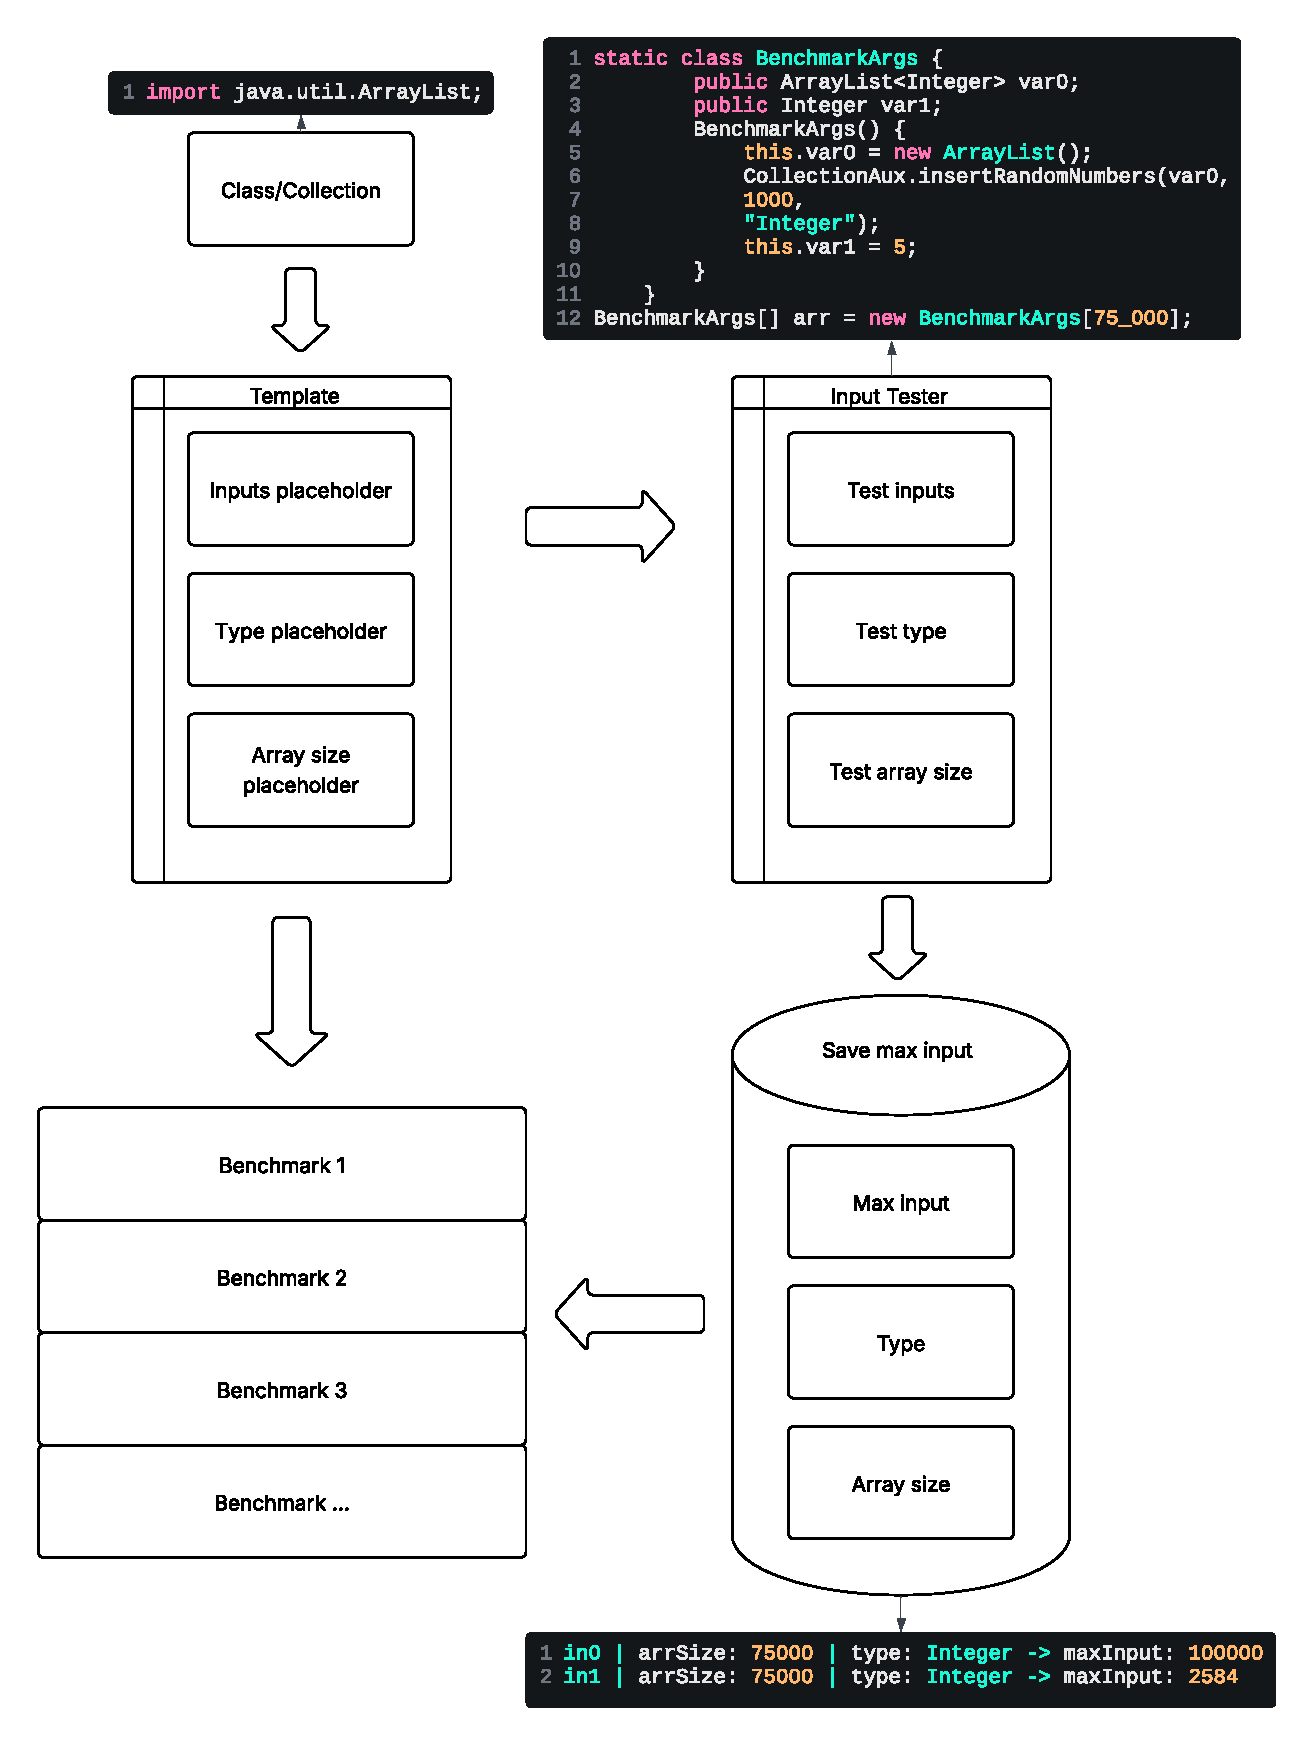
\includegraphics[width = 1 \textwidth]{figures/program_generator.pdf}
  \caption{Program Generator}
  \label{fig:program_generator}
\end{figure}

In order to be able to predict energy using ML models it is of course needed a lot of data, so the models can train, and the results can be analyzed. To obtain a considerable amount of data a program generator was built.
The program generator works alongside with Java Spoon to make it the more general as possible allowing custom programs to be mass generated.
The generator works for custom Java classes or for some collections (Lists, Sets, Maps), and it can be called to analyze all the public methods of the class or just specific ones.

\subsection{Template Creation} \label{sec:work_stage1_template_creation}


\FloatBarrier


\begin{minted}[linenos, fontsize=\small, frame=none, bgcolor=white,breaklines=true,breakanywhere=true]{java}

package com.generated_progs.ArrayList_add_java_lang_Object_;
import com.template.aux.CollectionAux;
import com.template.aux.TemplatesAux;
import java.util.ArrayList;
public class ArrayList_add_java_lang_Object_ {
    public static void main(String[] args) throws Exception {
        int iter = 0;
        try {
            BenchmarkArgs[] arr = new BenchmarkArgs["numberOfFunCalls"];
            populateArray(arr);
            TemplatesAux.sendStartSignalToOrchestrator(args[0]);
            TemplatesAux.launchTimerThread(1100);
            iter = computation(arr, arr.length);
        } catch (OutOfMemoryError e) {
            TemplatesAux.writeErrorInFile("ArrayList_add_java_lang_Object_", "Out of memory error caught by the program:\n" + e.getMessage());
        } catch (Exception e) {
            TemplatesAux.writeErrorInFile("ArrayList_add_java_lang_Object_", "Error caught by the program:\n" + e.getMessage());
        } finally {
            TemplatesAux.sendStopSignalToOrchestrator(args[0], iter);
        }
    }

    static class BenchmarkArgs {
        public ArrayList<changetypehere> var0;

        public changetypehere var1;

        BenchmarkArgs() {
            this.var0 = new ArrayList();
            CollectionAux.insertRandomNumbers(var0, "ChangeValueHere1_changetypehere", "changetypehere");
            this.var1 = "ChangeValueHere2_changetypehere";
        }
    }

    private static void arrayList_add_java_lang_Object_(ArrayList var, changetypehere arg0) {
        var.add(arg0);
    }

    private static int computation(BenchmarkArgs[] args, int iter) {
        int i = 0;
        while (!TemplatesAux.stop && i < iter) {
              arrayList_add_java_lang_Object_(args[i].var0, args[i].var1);
               i++;
        }
        return iter;
    }

    private static void populateArray(BenchmarkArgs[] arr) {
        for (int i = 0;i < "numberOfFunCalls";i++) {
          arr[i] = new BenchmarkArgs();
        };
    }

    private String input1 = "ChangeValueHere1";

    private String input2 = "ChangeValueHere2";
}


\end{minted}


The first step to generate multiple programs is to first create an intermediate template capable of holding the necessary code that will later be used for energy profiling.

The program generator starts by reading a custom Java file (or just access the Lists, Sets, Maps classes), and using Spoon it finds every public method available in the provided class. If it is needed to analyze a specific method, the generator will search in the class for every method with the name requested. Then it has access to all the public methods in the class and what parameters they receive.
Since it has access to the whole custom class, it can see how its constructors are called, and use them if any of the methods parameters requires. It recursively calls constructors if needed, making it very versatile to use. 

After identifying the methods that will be targeted, it starts by creating templates for each of them. 

Template important features

\begin{itemize}

  \item Input placeholders: Placeholders that will be later changed with real values for inputs, in this case inputs are variable values. 

  \item Type placeholder: Placeholders that will later be replaced with Java wrapper classes.
  
  \item \textcolor{blue}{Array Size placeholder: Placeholder that will later be replaced with the value of an array size. (This array will be explained in the next section)}. 

\end{itemize}

Also, the template is structured so that the programs will work in harmony with the Orchestrator, that will extract the energy profile for each program (next section), so when the placeholders are replaced with actual values, the orchestrator can run the program, and communicate with them.

\begin{listing}[H]
\begin{minted}[linenos, fontsize=\small, frame=none, bgcolor=white,breaklines=true,breakanywhere=true]{java}
static class BenchmarkArgs {
        public ArrayList<changetypehere> var0;

        public changetypehere var1;

        BenchmarkArgs() {
            this.var0 = new ArrayList();
            CollectionAux.insertRandomNumbers(var0, "ChangeValueHere1_changetypehere", "changetypehere");
            this.var1 = "ChangeValueHere2_changetypehere";
        }
    }
\end{minted}
\caption{Example of variable placeholders creations}            
\label{lst:var_placeholders}
\end{listing}

The template creates a class that holds the necessary variables the method needs to run, \ref{lst:var_placeholders} shows an example of the variables that need to be created to run the method List.add(Object). First it creates the list with the smallest constructor possible, then if the variable is a collection (List, Set, Map) it calls a custom-made method that populates collections with random values of a given type, and then it starts creating variables of parameters that the method List.add(Object) uses. The placeholder "ChangeValueHere1" will change to a random number, it contains a number ("1") because it represents the input number of the method that will later help the model training understand how inputs can affect energy consumption. The placeholder "changetypehere" later changes to a type.

It is worth mentioning that the types used by the generator are the Java wrapper classes, which are object representations of the primitive types. Using these types it is possible to achieve a more general generator, as every program can use them and if other custom types were used it would make the generator more complex and not general.

What mostly differs from template to template is the number of variables used, because different methods have different parameters, so the template can have more or less input placeholders, also the type placeholder changes according to the methods types and parameters.


Creating the template for each method allows cutting off time of the program generation by only having to replace values of the placeholders instead of needing to create the whole program all over again, since the programs for the same method only differ in inputs, types and array size, maintaining all the structure.

\subsection{Input Tester} \label{sec:work_stage1_input_tester}

A very important aspect of the program generator is the inputs it generates. Every method works differently, receives different parameters, and even when changing the values of these parameters, the method can behave completely different. So, this generator has an intermediate step, between the creation of the template and creating multiple programs, it finds the maximum size the input parameters should receive. Knowing the maximum size the different parameters can have is very important as it needs to be big enough, so the energy profiles can be abundant, but not to big so that the programs start to get out of memory or taking too much time to complete.
The input search works by using binary search. It has limits on the inputs (1-100,000) and it starts by trying to run the program with the half of the max input which is 50,000. Then it runs the program for maximum of 10 seconds (timeout also defined by us) and waits for the exit code of the program, if it is an error code it will lower the input by half again, of it is a normal finish code, it will increase the input by half. This operation is done until the maximum value for the input is found. If the method that is being tested has more than one input, the input tester, first sets all the input values to 1 and then starts the binary search individually for each of the parameters one by one while leaving the other parameters with the value of 1. This avoids having to find multiple combinations of parameters which would increase the time complexity exponentially. Since the process of finding the max inputs is time-consuming, when the maximum value is found, the values of the input type, maximum value and order (if it was the parameter 1 or parameter 2 or parameter 3) are stored in a file, so if the actual programs later generated are not stored, using this files they can be quickly generated.

\begin{tcolorbox}[title=Example: Input Testing Process for \texttt{List.add(index, Element)}, colback=gray!5!white, colframe=gray!75!black, fonttitle=\bfseries, breakable]

Consider analyzing the \texttt{add} method of a list with the following parameters:
\begin{itemize}
    \item \texttt{arg0}: Size of the list (integer)
    \item \texttt{arg1}: Index at which to insert the new value (integer)
    \item \texttt{arg2}: Value to be added (integer)
\end{itemize}

\textbf{Step 1 – Varying \texttt{arg0} (list size):}

\begin{itemize}
    \item Iteration 1: \texttt{arg0 = 25,000}, \texttt{arg1 = 1}, \texttt{arg2 = 1}
    \item Iteration 2: \texttt{arg0 = 12,500}, \texttt{arg1 = 1}, \texttt{arg2 = 1}
    \item Iteration 3: \texttt{arg0 = 6,250}, \texttt{arg1 = 1}, \texttt{arg2 = 1}
    \item $\vdots$
    \item Final Iteration: \texttt{arg0 = 1,700}, \texttt{arg1 = 1}, \texttt{arg2 = 1}
\end{itemize}


\textbf{Step 2 – Varying \texttt{arg1} (index):}

\begin{itemize}
    \item Iteration 1: \texttt{arg0 = 1}, \texttt{arg1 = 25,000}, \texttt{arg2 = 1}
    \item Iteration 2: \texttt{arg0 = 1}, \texttt{arg1 = 12,500}, \texttt{arg2 = 1}
    \item $\vdots$
    \item Final Iteration: \texttt{arg0 = 1}, \texttt{arg1 = 0}, \texttt{arg2 = 1}
\end{itemize}

{Note: Since the list size (\texttt{arg0}) remains 1, the maximum valid index (\texttt{arg1}) is constrained to 0. This reveals a limitation in the input testing approach.}
\vspace{5mm}
\textbf{Step 3 – Varying \texttt{arg2} (value to be added):}

\begin{itemize}
    \item Iteration 1: \texttt{arg0 = 1}, \texttt{arg1 = 1}, \texttt{arg2 = 25,000}
    \item Iteration 2: \texttt{arg0 = 1}, \texttt{arg1 = 1}, \texttt{arg2 = 37,500}
    \item $\vdots$
    \item Final Iteration: \texttt{arg0 = 1}, \texttt{arg1 = 1}, \texttt{arg2 = 100,000}
\end{itemize}

\textbf{Final stored input limits:}
\begin{itemize}
    \item \texttt{arg0} — \texttt{integer} — \texttt{1,700}
    \item \texttt{arg1} — \texttt{integer} — \texttt{1}
    \item \texttt{arg2} — \texttt{integer} — \texttt{100,000}
\end{itemize}

\end{tcolorbox}

The fact that the input has a range of 1 to 100,000 it allows using binary search which makes the search much faster than linear search.
Nevertheless, the input search does not come without some limitations. First it is constrained to identifying valid input values within the range of 1 to 100,000. Throughout this project we dealt frequently with lists and collections, which require a minimum size of 1 to function correctly. Although this value can be changed in the future, for now it ensures compatibility with most common data structures. The higher bound of 100,000 was chosen due to practical experience, as larger input values would lead to higher execution times and memory crashes. Another limitation is on how the input handles multiple parameter methods. During its search for a valid input, it needs to fix all the other parameters that is not searching, with a default value (typically 1). This approach simplifies the testing process and improves efficiency by avoiding the exponential complexity of testing all possible parameter combinations. However, it will introduce limitations in cases where the parameters are interdependent, which can lead to not estimating the real highest input possible. The process also has a timeout of 10 seconds. This threshold was empirically selected to balance precision and practicality, based on our needs and available hardware.
Despite these limitations, the input search plays a crucial role in ensuring that the program generator produces viable test cases. By identifying input ranges that are both valid and computationally achievable, it reduces the unusable generated programs (e.g., due to timeouts or crashes), and maximizing the number of generated programs, that can be used for energy profiling.



\subsection{Program Generation} \label{sec:work_stage1_program_generation}

Finally, when the templates are created, and the maximum inputs are found the program generation can finally begin. This part consists on picking every template created and replacing the placeholder values with actual values created by a random number generator.

It starts by looping through the types and changing them to the Java wrapper classes, then it loops through the array size, \textcolor{blue}{{again this value will be explained in the next section}}. Lastly, it loops through the input sizes determined by the input tester and can repeat this process a configurable number of times. By increasing the number of iterations, results in more programs being generated with random inputs, constrained by the previously identified input bounds.

This process easily generate thousands of programs which are crucial to train machine learn models that are able to predict energy consumption. When generating programs, a number is chosen to balance the requirements for effective model training while minimizing the time spent on input testing and collecting energy profiles. Afterwards, that the programs are ready to be compiled and used.



\section{Stage 2: Orchestrator} \label{sec:work_stage2_orchestrator}

Having all the programs generated, it is possible to move to the next stage. Gathering the energy profiles for each of the generated programs. This step is necessary, of course, because to give energy consumption estimates, first it is necessary to obtain energy profiles~\cite{10.1145/2884781.2884869,8816747}, so the machine learning models can obtain the most accurate results possible. To make this task as easily as possible, a process was implemented, so the task was made automatically. 

Note: Although this part was developed chronologically before Section \ref{sec:work_stage1_program_generator}, it is presented as Stage 2 to reflect the logical structure of the system: programs must first be generated before they can be energy profiled. For this reason, the program generator templates are designed to integrate directly with the orchestrator.

As described in \ref{sec:background_energy} there are several tools capable of performing dynamic energy measurements. In our case we choose PowerJoular, it has good features that caught our attention, for example being a command line tool that could be easily integrated in almost every programming language, it stores the energy used in a CSV file (easy to work with), capable of only reading energy of running processes and so on, as explained before. So, PowerJoular is the tool that will measure the energy of our programs.

Since PowerJoular is a command line tool, it is launched as a process and then it can be killed whenever needed because it is a process as well. This allows to measure not only programs/processes energies but have a more precise measurement, as it is possible to call PowerJoular to measure a specific computation and then kill it when the computation is finished.

With all of this in mind a process was built. The process uses an orchestrator that is responsible for invoking the target program and the measurement tool (PowerJoular) to accurately measure the energy consumption of the program or the specific computation being analyzed within it.


The workflow of this step can be described as follows:

\begin{itemize}
  \item The orchestrator launches a command to start the target Java Program and waits a signal.
  \item The Java program starts and setup the necessary elements to run (creating all the variables, reading/writing files, etc.) and then before starting the computation it wants to measure, it sends a start signal to the orchestrator to start monitoring, and waits for 100 milliseconds.
  \item The orchestrator receives the start signal and reads the PID and number of runs the target computation is going to take, which is stored in a file during the target program setup. And, finally, it starts PowerJoular using that PID. Then it waits for the stop signal.
  \item The Java program will run until it finishes the computation and then, send a stop signal back.
  \item The orchestrator on receiving the stop signal, first stops PowerJoular and then stops the target program, if needed. Then it parses the target program to extract its features, combines them with the energy information stored in the files created by PowerJoular, stores it in a CSV file and displays the energy on the screen.
\end{itemize}



\begin{comment}
\section{Step 1: Energy Profiling} \label{sec:work_step1_energy_profiling}

To give energy consumption estimates, first it is necessary to obtain energy profiles~\cite{10.1145/2884781.2884869,8816747}, so the inference function can obtain the most accurate results possible. The goal in this step is to first obtain energy profiles of collections and APIs that are widely used, break them down to their smallest functions, and understand their energy behavior. From there, it is possible to build from these granular functions to more complex and interconnected functions, ultimately covering the entire API set in detail. So whenever an API call is detected in the code, pre-built energy profiles are already available for it.
For that, a process was created in order to efficiently obtain the energy usage of code snippets.
The process uses an orchestrator that is responsible for invoking the target program and the measurement tool (PowerJoular) to accurately measure the energy consumption of the program or the specific computation being analyzed within it.

The workflow of this step can be described as follows:

\begin{itemize}
  \item The orchestrator launches a command to start the target Java Program and waits a signal.
  \item The Java program starts and setup the necessary elements to run (starting threads, reading/writing files, etc.) and then before starting the computation it wants to measure, it sends a start signal to the orchestrator to start monitoring, and waits for 100 milliseconds.
  \item The orchestrator receives the start signal and reads the PID and number of runs the target computation is going to take, which is stored in a file during the target program setup. And, finally, it starts PowerJoular using that PID. Then it waits for the stop signal.
  \item The Java program will run until it finishes the computation and then, send a stop signal back.
  \item The orchestrator on receiving the stop signal, first stops PowerJoular and then stops the target program, if needed. Then it parses the target program to extract its features, combines them with the energy information stored in the files created by PowerJoular, stores it in a CSV file and displays the energy on the screen.
\end{itemize}

The process described is responsible for generating energy profiles of various programs and storing them in a CSV file, which will be used later for training the ML model.

This allows for more precise energy measurements, avoiding reading the JVM startup, and focusing only on the computation between the signals. The workflow is more clearly illustrated in Figure \ref{fig:orchestrators_process}.

\begin{figure}
  \centering
  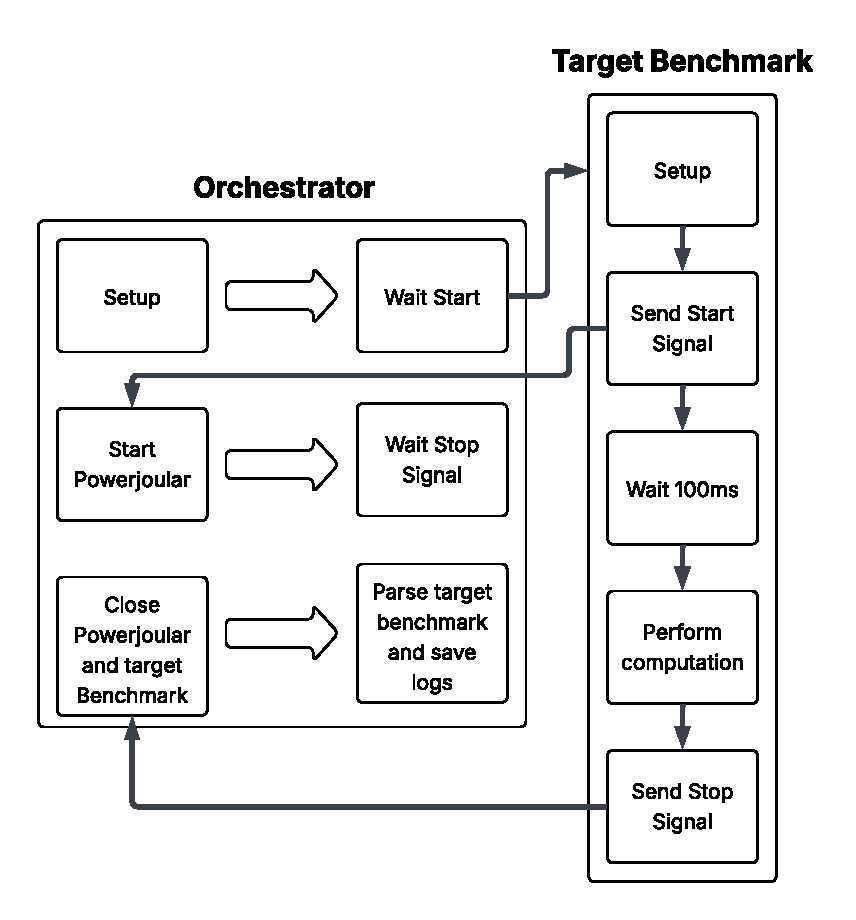
\includegraphics[width = 0.4 \textwidth]{figures/orchestrators_process.pdf}
  \caption{Orchestrator Workflow}
  \label{fig:orchestrators_process}
\end{figure}

The same workflow will be repeated across multiple machines to gather data from as many locations as possible. This approach ensures that the model developed in the next step will generate accurate outputs applicable to a wide range of machines and scenarios.


\section{Step 2: Energy Inference Function} \label{sec:work_step2_energy_inference_function}

\begin{figure}%[h]
  \centering
  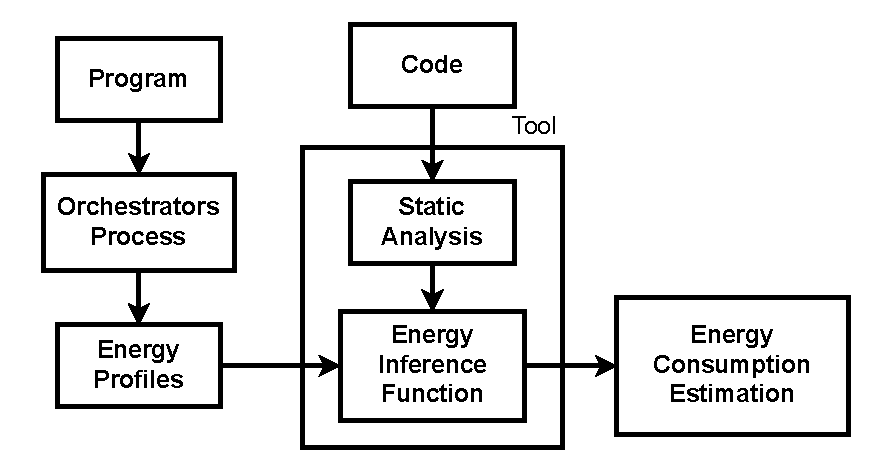
\includegraphics[width = 0.4 \textwidth]{figures/energy_inf_fun.pdf}
  \caption{Energy Inference Function}
  \label{fig:energy_inference_function}
\end{figure}

The inference function will receive as input the energy profiles obtained previously and the code that the developer wants to analyze. On receiving the code, static analyzes will be used in order to inspect the code using a Java parser (Spoon), which will provide the AST. Later this AST will be used to feed a machine learning model with the return types of the function, parameters used, loops and so on, alongside with the energy profiles. After that the model will output the estimated energy values to be displayed to the developer.
As explained in \ref{sec:background_machine_learning}, there are several ways of implementing an ML model. In this particular case, supervised ML is the best approach as it allows to train the model on previously collected energy profiles that contain the code and the energy consumed for that code. With these in mind, it is possible to test different algorithms, like the ones described in \ref{sec:background_machine_learning}, to achieve the best estimation possible.


The model will be trained using a variety of energy profiles and code inputs from different devices to achieve the most accurate energy estimates possible. This approach will improve its accuracy across devices with different hardware and software configurations.
The estimation will be the total energy used by the program, the total energy used for each function and the snippets of the function that spend the most energy.
The Figure \ref{fig:energy_inference_function} helps to visualize the function.
\end{comment}


\section{Step 3: Implementation and testing} \label{sec:work_step3_implementation_and_testing}

Once the main components of the tool are built, they need to be assembled into the extension. When using it, the developers should be able to see the total energy estimate of their code in the IDE, and it should also show the estimates for each function and its most energy consuming lines.
The estimate alone may be enough to understand if the code is high or low in energy consumption, for example, if the developer has two implementations of the same function and they both give different values, it may be easy to understand which one consumes the most. However, this may not always be the case, so the tool will also provide some information to help the developer know how good or bad the energy efficiency of the code is.

Another important step is to test and ensure that the tool performs as expected on most machines, delivers the most accurate estimations possible, and undergoes a final comparison with other tools to evaluate its effectiveness.
